\section{Föremål}
\subsection{Borfima}
\label{itm:Borrfima}
%
En \textit{borfima} är en läderpåse innehållande blod, fett, äggvita, tupp-blod och ris. Denna borfima tillbads av \textit{Leopardsällskapet}, och skulle ge innehavaren lycka och framgång, men till ett högt pris. Borfiman behövde nämligen ``matas'' så att säga. Den skulle fyllas på med kött, fett och blod från människor, specifikt ifrån innehavarens egna familj. Om borfiman var nöjd gav detta innehavaren framgång, men var den inte det drog den med sig olycka. Det är mycket få som vet detta, men en borfima är egentligen inget mer än en avbild av \textit{Shub-Niggurath}, en perverterad fruktbarhetsgudinna som har makten att förvränga verkligheten och ge sin tillbedjare det den vill ha. När borfiman behövde matas bad innehavaren en underhuggare i Leopardsällskapet att mörda en familjemedlemm till innehavaren och ta med dennes kropp till en offerplats. Där, framför en staty föreställande en man med leopardhuvud, offrades kroppen av medlemmarna i Leopardsällskapet, borfiman matades och medlemmarna åt av kroppen. En väl omhändertagen borfima kan låta en innehavare åkalla följande besvärjelser.
%
\begin{itemize}
	\item Köttets Skydd
	\item Nyogathas Grepp
	\item Smälta Kött
	\item Åkalla anden av en leopard.
\end{itemize}
%
Med mer kunskap och studier kan borfiman även användas för att åkalla \textit{Shub-niggurath}. Denna åkallan måste göras under en klar natthimmel, med borfiman och frammför ett leopardaltare. När den mörka gudinnan är åkallad ska borfiman, som fungerar som ett människooffer, sprättas upp och tömmas över altaret.

\subsection{Leopardkniv}
\label{itm:Leopardkniv}
%
\begin{figure}[h]
\centering
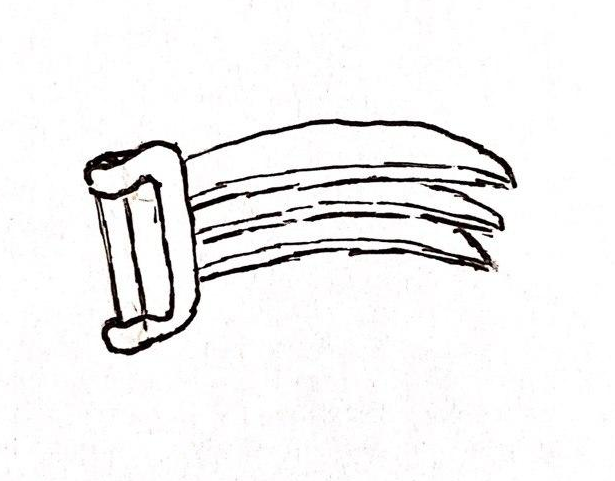
\includegraphics[width=8cm]{LeopardKniv.png}
\caption Leopardkniv
\end{figure}
%
En \textit{Leopardkniv} är ett vapen som primärt används av Leopardsälskapet för strid och för att mörda sina offer. Prof. Olofsson har fått en som en gåva ifrån en medlem i sällskapet, som han använde för att offra sin systerdotter. Den ligger nu i professorns nattygsbord i hans villa. Kniven har tre krökta blad och ett grepp vinkelrätt emot dess blad.
